\documentclass{article}
% hiermit werden alle packages in eine separate .tex datei ausgeladen
% zum Einblenden von Grafiken
\usepackage{graphicx}
% ändert die automatisch generierten wörter (inhaltsverzeichnis etc.) zu deutsch. 
% default ist englisch, also einfach das includepackage löschen.
\usepackage[german]{babel}
% um Grafiken gezielt anzuzeigen mit /begin{figure}[H] /end{figure}
\usepackage{float}
%Quelltexthighlighting, integration dessen nicht als rastergrafik, sondern skalierbar
\usepackage{minted}

\usepackage[top=2cm, bottom=2cm, outer=0cm, inner=0cm]{geometry}
\usepackage[pages=some]{background}



\begin{document}

    % command um ein hintergrundbild für alle seiten einzufügen, random kommentar im command um random leerzeichen raus zu kriegen
    % außerdem transparent mit hilfe eines weiteren packages
    %außerdem versch. hintergr. für gerade und ungerade seiten, wieder ein neues package
    \AddToShipoutPicture{%
        \ifthenelse{
            \isodd{
                \value{page}}
        }
        {%
            \transparent{0.2}
\includegraphics[width=\paperwidth, height=\paperheight]{graphics/backg02.jpg}
        }
        {%
            \transparent{0.2}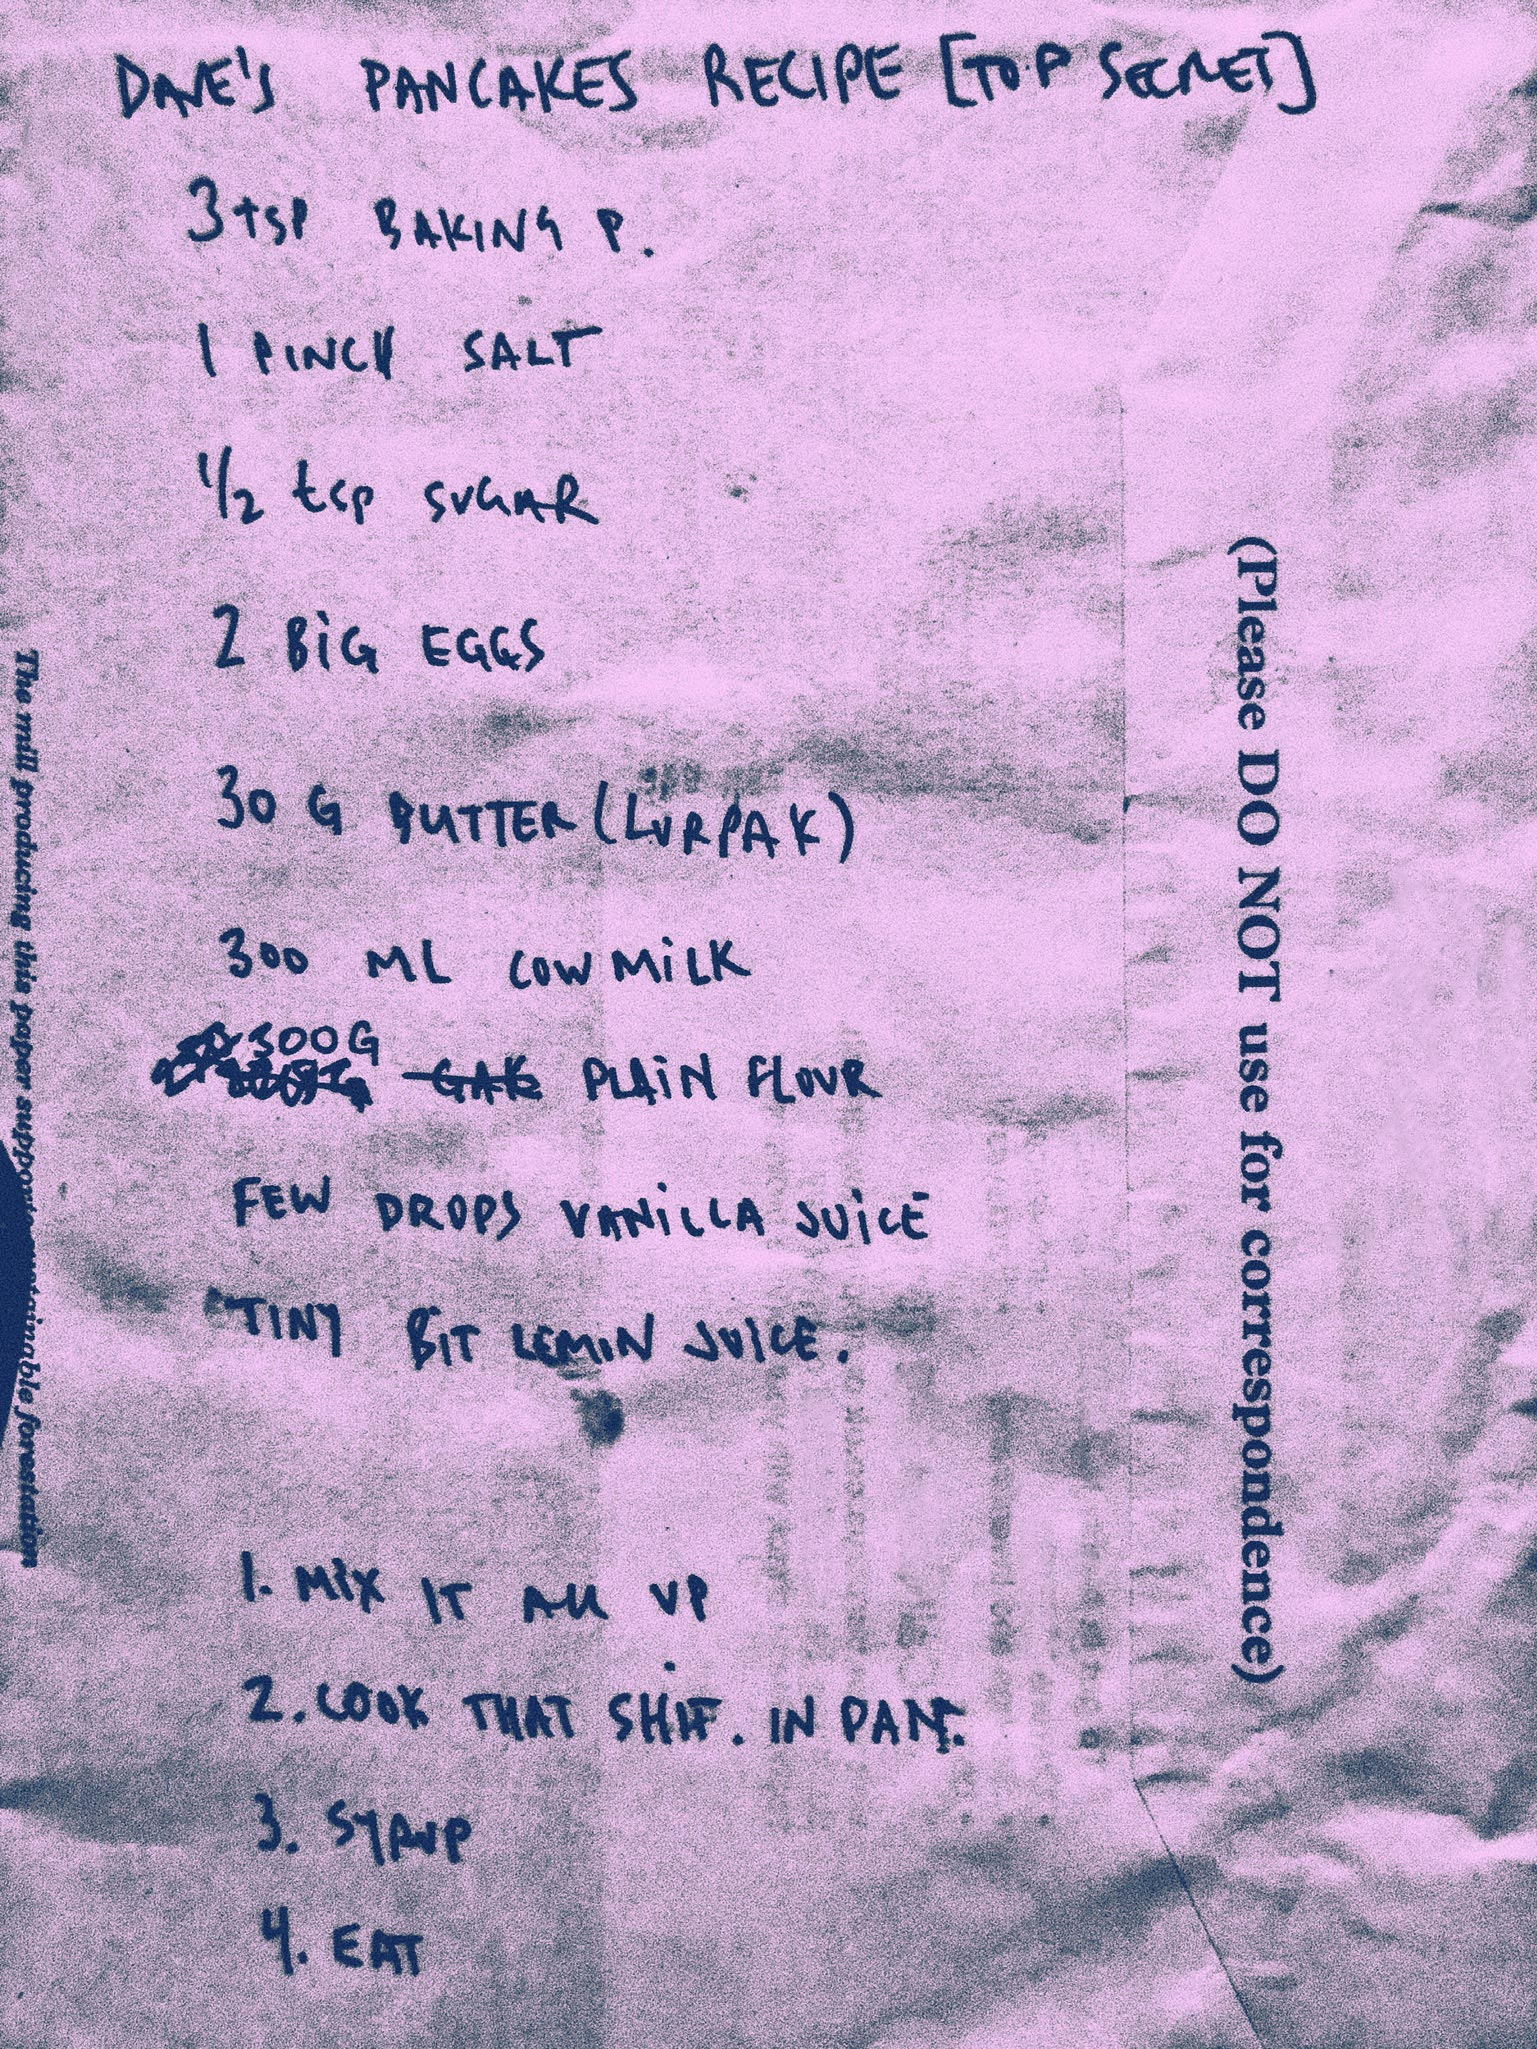
\includegraphics[width=\paperwidth, height=\paperheight]{graphics/DAVES_PANCAKES_RECIPE.jpg}
        }
    }

    
    
    

    %\newpage

    

    \begin{center}

        
\includegraphics[width=0.5\paperwidth]{graphics/logo black.jpg}
        \vspace{20mm}

        %mit huge können sachen sehr groß geschrieben werden, allerdings muss danach ein normalsize folgen
        % textsc, um ne nice überschrift mit kapitälchen zu schreiben
        \Huge{\textsc{Deckblatt}}
        \normalsize
    
        % und noch ein leerzeichen in das ding reinfeuern
        \vspace{20mm}
    
        % eine tabelle, um coole sachen geordnet darzustellen
        \begin{tabular}{r c l}
            Erstprüfer & Singer & Jürgen \\
            Zweitprüfer & Ackermann & Daniel \\
            Abgabedatum & 18. August & 2020 \\
        \end{tabular}
    
        % vfill für cooles einrichten einzelner elemente auf der seite.
        \vfill
        \begin{tabular}{r c l}
            Erstprüfer & Singer & Jürgen \\
            Zweitprüfer & Ackermann & Daniel \\
            Abgabedatum & 18. August & 2020 \\
        \end{tabular}
    
    
        
        % ohne das letzte vfill würde tabelle nach ganz unten eingerückt werden
        % \vfill 
    
    \end{center}

    \tableofcontents

    \renewcommand{\listoflistingscaption}{Listingverzeichnis}
    \listoflistings

    \section{Der Anfang vom Anfang.}
    Der Text ist \underline{\textit{\textbf{"verhext"}}}, braucht kein Slash und keine Klammern, 
    das ist der Hammer(n).

    \enquote{Und dieser Text ist umgeben von Anführungszeichen.}
    
    
        Die Abbildung \ref{fig:DAVES_PANCAKES_RECIPE} zeigt das erleuterte Rezept
        in größerem Detail. 

        % line break mit leerzeichen zwischen den zeilen! so easy!
        1.) zutaten

        2.) bearbeitungsweise

        \begin{figure}[H]
            \centering
            % error 'overfull' = bild zu groß für platz, fixed indem man width auf das 0.x Fache anpasst (hier 0.5) 
            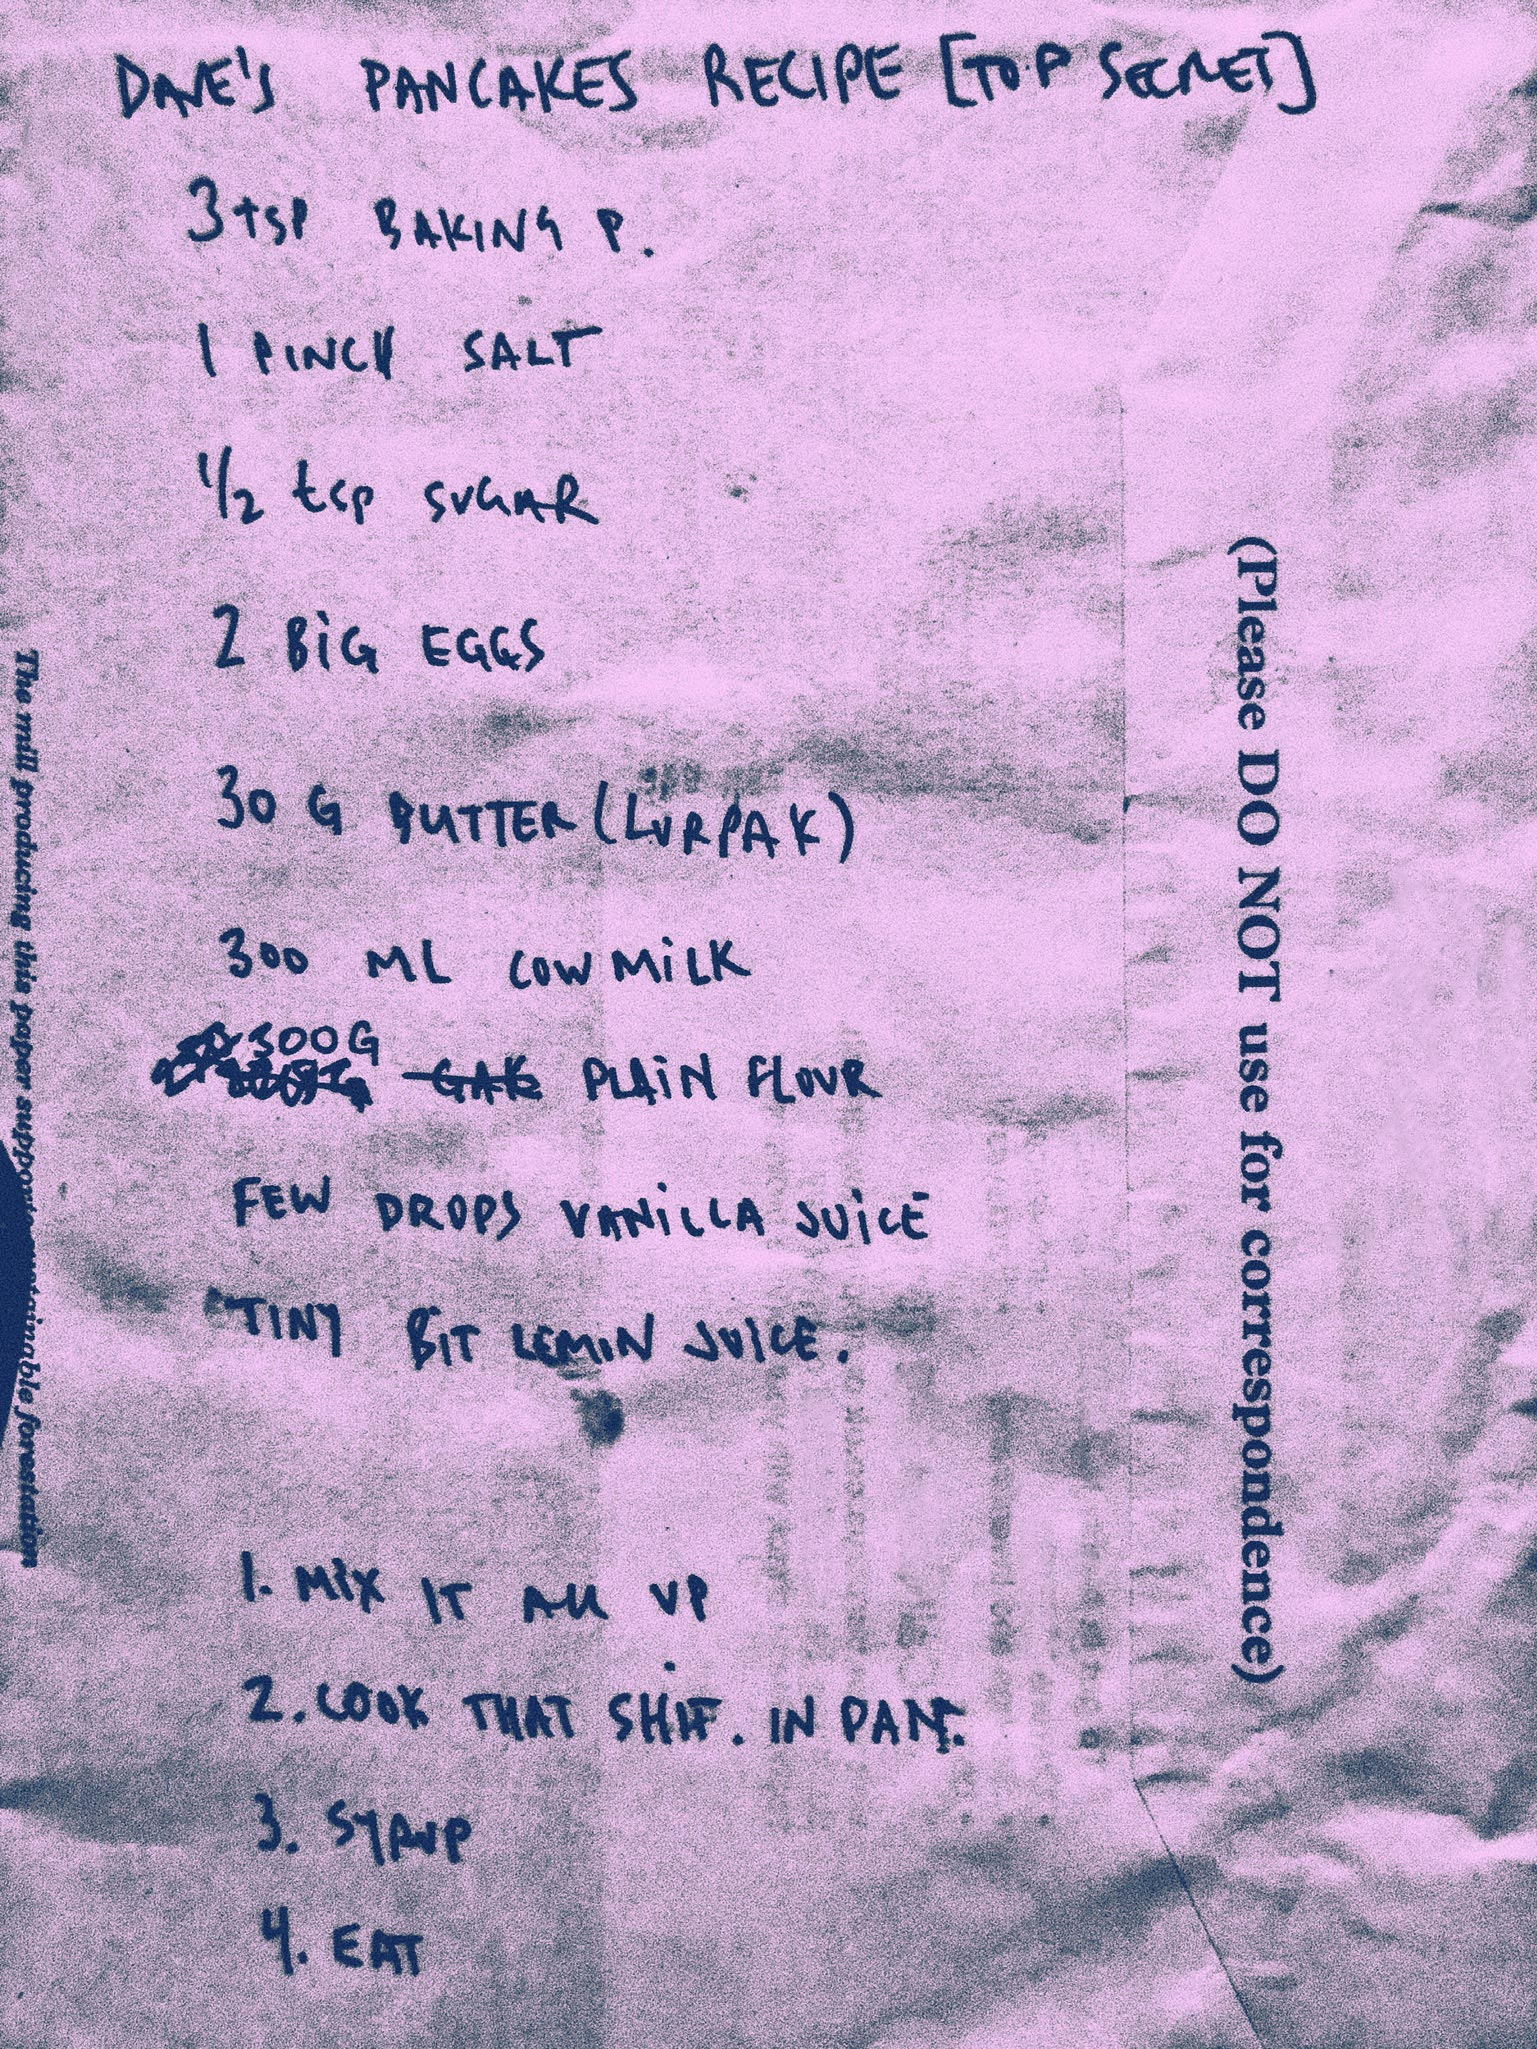
\includegraphics[width=0.5\linewidth]{graphics/DAVES_PANCAKES_RECIPE.jpg}
            \caption[cooles rezept]{Abbildung zeigt details}
    
            
            %mit label werden grafiken in texts referenziert
            \label{fig:DAVES_PANCAKES_RECIPE}
        \end{figure}
        
        \subsection {erstes Unterkapitel vom ersten Kapitel.}
        Badabing Badabum.

            \subsubsection{we need to go deeper!}

                \paragraph{insert dumb Inception joke inside the paragraph. it won't go deeper though.} 
                   
                    \subparagraph{subparagraph as smallest unit of text.}


                    
        
    \section{Was ist ein Problem?} \label{kapitel_02}
you already know. wow. 
\begin{listing}[h]
    %caption wird benötigt, um das lisiting in das verzeichnis aufzunehmen, same mit abbildungen
    \caption[Quelltext]{beschreibe den Quelltext hier.}
% linenos -> numeriert zeilen, frame=lines -> grenzt code mit linien ab, fontsize -> schriftgröße, 
% firstnumber -> zeile, in der snippet anfängt, muss al erster parameter stehen
% unter den mathescape eingaben dann die gewählte sprache in {}
% verfügbare sprachen via pygmentize dokumentation 
\begin{minted}
    [
        firstnumber=5,
        frame=lines,
        framesep=2mm,
        baselinestretch=1.2,
        linenos
        ]
{java} 

package com.tutego.insel.ds.observer;

import java.util.*;

public class Party
{
  public static void main( String[] args )
  {
    Observer achim    = new JokeListener( "Achim" );
    Observer michael  = new JokeListener( "Michael" );
    JokeTeller chris  = new JokeTeller();

    chris.addObserver( achim );

    chris.tellJoke();
    chris.tellJoke();

    chris.addObserver( michael );

    chris.tellJoke();

    chris.deleteObserver( achim );

    chris.tellJoke();
  }
}

\end{minted}
    \label{lst:mein_Quelltext}
\end{listing}

Im Quelltext \ref{lst:mein_Quelltext} sieht man einen Ausschnitt eines Java Quelltextes.
    \section{kapitel 3}

\begin{center}

    %mit huge können sachen sehr groß geschrieben werden, allerdings muss danach ein normalsize folgen
    % textsc, um ne nice überschrift mit kapitälchen zu schreiben
    \Huge{\textsc{Tabelle}}
    \normalsize

    % und noch ein leerzeichen in das ding reinfeuern
    \vspace{20mm}

    % eine tabelle, um coole sachen geordnet darzustellen
    \begin{tabular}{r c l}
        Erstprüfer & Singer & Jürgen \\
        Zweitprüfer & Ackermann & Daniel \\
        Abgabedatum & 18. August & 2020 \\
    \end{tabular}
\end{center}
    
        
    \newpage

    \listoffigures

\end{document}




